We built ranking models for Sports, Finance and News stream respectively. We collected two weeks of user action data from these streams. These two week data was used as training. We also collected one more week data as test. The method of data collection has been described in Section~\ref{sec:phase2}. Sports, Finance and News are big streams. Under them there are small streams such as NFL,NBA,MLB from Sports. These structure is  shown in Fig.~\ref{hierarchy}. Data distribution are shown in Table.~\ref{data distribution}. The table shows the number of clicks and views for different properties in our training and test data. 



\begin{table}
\begin{center}
\caption{Click data distribution}
\begin{tabular}{|c|c|c|c|c|c|c|}\hline
 &  \multicolumn{3}{c|}{training} & \multicolumn{3}{c|}{test} \\ \hline
property     & click & view & total & click & view & total\\ \hline
Sports &  108K & 1.5M  & 1.6M & 12K & 178K & 191K \\ \hline
NFL &   20K & 328K  & 347K & 1.5K & 21K & 22K \\ \hline
NBA  &  7K & 66K & 72K & 649  & 8K & 9K \\ \hline
MLB & 7K & 9K & 95K & 971 &14K & 15K \\ \hline
Finance & 57K & 779K  & 836K & 5K &73K & 79K \\ \hline
News & 109K & 1.4M &1.5M  &14K &207K &221K \\ \hline
\end{tabular}

\end{center}
\end{table}
\label{data distribution}

GBDT is our learning method of choice.  The comparision between GBDT and linear regression under different feature size  are shown in Table~\ref{phase2sum}. The base model was made by linear regression with features from Phase 1 (equal to "flat gmp'' as in Table~\ref{tag:phase1exp}). Note experiments on Phase 1 and Phase2 used distinct training set and test set. Hence, the numbers shown on Table~\ref{phase2sum} and Table~\ref{tag:phase1exp} are not aligned. Two GBDT models' results  are shown. One used phase 1 features and the other used  Phase 2 features as described in Section~\ref{sec:phase2}, which has 14 features in total.  The same algo was applied into three properties: Sports, Finance and News.  The linear Base models gave the worst results. The GBDT with Phase 2 features derived the best results. The metric is AUC.  


\begin{table}
\caption{Comparision of Phase 2 ranking models}
\begin{tabular}{|c|c|c|c|}\hline
             & Sports & Finance & News \\ \hline
Base (linear phase1 feature) & 0.56 & 0.53 & 0.56 \\ \hline 
GBDT(Phase 1 feature)  & 0.59& 0.62& 0.58 \\ \hline
GBDT(Phase 2 feature) & 0.64 & 0.66 & 0.62 \\ \hline
\end{tabular}

\label{phase2sum}
\end{table}


Intuitively, we would assume better results could be derived if each stream uses its own model. Actually, we found this assumption was right if the difference of streams are very different in content type such as Sports, Finance and News. We regard these streams as heteogenerous streams. We should build a separate model each for heteogenerous streams. But this assumption is incorrect for homogeneous steams by our experiments such as NFL,NBA and MLB, which are sub-streams of Sports.  To show this, we trained a general model using all sports data, and a dedicated model for each sub-stream using only the data from each sub-stream. Accordingly, we test the models on test data from different streams. The results are shown in Table~\ref{tab:substream}. 

\begin{table}
\caption{Substream evaluations}
\begin{tabular}{|c|c|c|c|c|} \hline
    \diaghead{\theadfont training  test data}{training \\ data}{test  data}   & Sports & NFL & NBA & MLB \\ \hline
    Sports & 0.636 &0.629 &0.662 &0.705 \\ \hline
    NFL & - & 0.610 & - & - \\ \hline
    NBA & - & - & 0.645 & \\ \hline
   MLB & - & - & - & 0.676 \\ \hline
   with srcspaceid  & 0.642  & 0.635 &0.689 & 0.725 \\ \hline
\end{tabular}

\label{tab:substream}
\end{table}

We found the model trained on all sports data performed better than dedicated models. 
We interpreted this as that using all data can have rich feature distribution while  feature distribution is biased for sub-stream streams. Simply increasing training data size can't satisfy rich feature distribution.  Actually, the training data sizes we used for sub-stream models  were sufficient to make maximal performance. As shown in Fig.~\ref{fig:curve}, it is a training curve which shows the trend of  AUC change on the same test set as increasing training data size. The training data size is large enough to make the maximal results, which proves increaing more training data size does not help.  

\begin{figure}
\caption{Test data metrics as increasing sub-stream training data size}\label{fig:curve}
%\centering 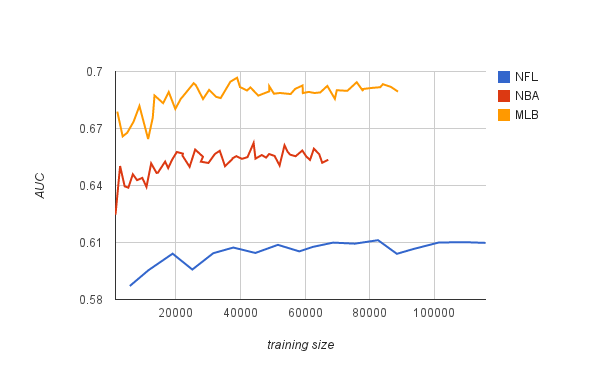
\psfig{file=training-curve.png,width=3.3in,}
\centering
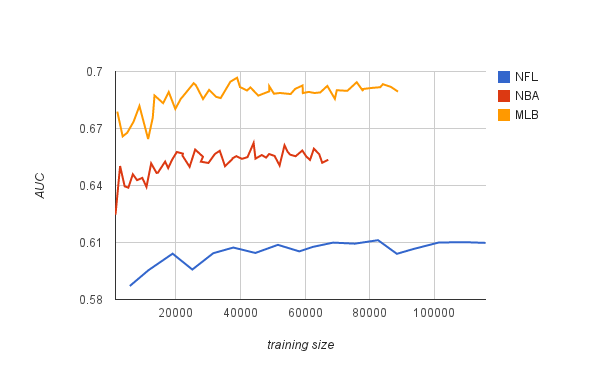
\includegraphics[width=3.5in]{training-curve.png}

\end{figure}

We found using srcspaceid as feature can improve substream ranking. This is a unique feature for multiple stream ranking. The feature is a category feature which is supported by our in-house GBDT.  The decision tree can be split at node with logic as  $srcspaceid \in \{NFL,NBA\}$.  The model with this features was trained on all sports data.  The results are even better  than using all sports data. The results of using srcspaceid is shown on the last line of  Table~\ref{tab:substream}.   We found this was a very useful feature. With it all streams' ranking are improved. 
 




  
 Ranking has to promote fresh contents.  However, if recency is not specifically treated,   many old articles can be ranked on the top of stream because old articles can accumulate higher popularity scores.  In the other hand, recency can't be over-promoted.  Ranking solely by document age is a very bad idea because this will show many low quality and irrelevant articles to users. Therefore, a ballance ranking between relevance and recency is considered.  Usually, there are two methods in handling recency. First as used in Phase 1, recency is boosted by applying an exponential age decay factor. Old age documents are punished.  Related works can be found in \cite{Li:2003:TLM:956863.956951,Metzler:2009:ISR:1571941.1572085}. Second,  use document age as features. Recency feature is integrated with other features. The importance of recency and relevance feature is completely determined by the training data and the algorithm. We tested the two methods. The results are shown in table~\ref{recency}.

\begin{table} 
\caption{ Recency evaluation }\label{recency}
\begin{tabular}{|p{50mm}|c|c|}\hline
     & AUC & age@top1 \\ \hline
Sports Base (Phase2 gbdt) &  0.64 & 10.3  \\ \hline
Sports (expontial age decay) & 0.58 & 7.5 \\ \hline
Sports (age as feature) & 0.66  & 8.3 \\ \hline \hline
%% Sports (age as feature) + expontial age decay & 0.62 & 6.5 \\ \hline  \hline
Finance Base & 0.66 & 6.6 \\ \hline
Finance (expontial age decay) & 0.60 & 4.6 \\ \hline
Finance (age as feature)  & 0.68 & 6.4 \\ \hline
%%Finance (age as feature) + expontial age decay & 0.64 & 4.2 \\ \hline
\end{tabular}

\end{table}

"age@top1" is the average document age (hour) of the first articles in the stream for all sessions. A session is the period from when a user comes to the site to when she leaves, or 30 minutes depending on which is shorter. The unit of this metric is hour. For example, the average document ages of Sports Base ranking is 10.3 hours.   The Base model is GBDT model with phase 2 features.     The model "expontial age decay"  applied expontial age decay on the results of the Base model like $e^{-\beta \Delta T}$ in Equation~\ref{practical SRQ}. The model "age as feature" used age as feature in GBDT. 
%%The final one "age as feature + expontial age decay" applied expontail age decay over the results from "age as feature".  This is an effort to boost recency
We found that using document age as a feature achieves better results than using expontial age decay: both AUC (relevance metric) and age@top1 are improved while expontial age decay resulted in a big relevance drop in terms of AUC.
The results are consistent for both Sports and Finance streams. 


We also did online user experience test (bucket test) to evaluate GBDT models (Table~\ref{bucket test}). We were able to do bucket test for Sports and Finance at the time. The models are compared to a linear model (as Phase 1). The bucket results were very excited. Both CTR and Dwelltime are improved more than double digits and the improvement is significant. 

\begin{table}
\caption{bucket test}
\begin{tabular}{|c|c|c|}\hline
             & CTR & Dwell time  \\ \hline
Base (Linear) &  - & -   \\ \hline 
Sports,GBDT(phase 1 feature)    & +6\% & +6\% \\ \hline
Sports,GBDT(Phase 2 feature) & +25\% & +21\% \\ \hline
Finance,GBDT(phase 1 feature)  & +3\% & +3\% \\  \hline
Finance,GBDT(Phase 2 feature) & +20\% & +18\%  \\  \hline
\end{tabular}

\label{bucket test}
\end{table}






